\documentclass[aspectratio=169,compress]{beamer}
  \useoutertheme[footline=authorinstitute,subsection=false]{miniframes}
  \useinnertheme{circles}
  \usefonttheme{default}

  \definecolor{palatinate}{RGB}{126,49,123}
  \definecolor{pale-palatinate}{RGB}{216,172,214}
  \definecolor{grey-palatinate}{RGB}{150,142,133}
  \definecolor{dirt-palatinate}{RGB}{159,161,97}
  \definecolor{blue-palatinate}{RGB}{0,99,136}

  \setbeamercolor*{palette primary}{fg=blue-palatinate}
  \setbeamercolor*{palette secondary}{fg=palatinate,bg=pale-palatinate}
  \setbeamercolor*{palette tertiary}{fg=white,bg=palatinate}
  \setbeamercolor*{palette quaternary}{fg=white,bg=dirt-palatinate}

  \setbeamercolor*{normal text}{parent=palette primary}
  \setbeamercolor*{footline}{parent=palette secondary}
  \setbeamercolor*{headline}{parent=palette tertiary}
  \setbeamercolor*{titlelike}{parent=palette secondary}

  \setbeamercolor*{structure}{parent=normal text}
  \setbeamercolor*{title in head/foot}{parent=headline}
  \setbeamercolor*{section in head/foot}{parent=headline}
  \setbeamercolor*{author in head/foot}{parent=footline}
  \setbeamercolor*{institute in head/foot}{parent=footline}

  \setbeamercolor{block title}{fg=white,bg=blue-palatinate}
  \setbeamercolor{block body}{parent=normal text,bg=pale-palatinate!5}

  \setbeamercolor{block title example}{fg=white,bg=dirt-palatinate}
  \setbeamercolor{block body example}{parent=normal text,bg=dirt-palatinate!5}

  \setbeamertemplate{blocks}[rounded][shadow=true]
  \setbeamertemplate{caption}[numbered]

  \setbeamerfont{footnote}{size=\tiny}
  % \setbeamertemplate{navigation symbols}{}
\usepackage[style=science,backend=bibtex]{biblatex}
  \bibliography{references.bib}
\usepackage[labelfont={footnotesize,it},textfont={footnotesize,it}]{caption}
\usepackage[utf8]{inputenc}
\usepackage{tikz}
  \usetikzlibrary{calc}
  \usetikzlibrary{external}
    \tikzexternalize[prefix=tikz/]
  \usetikzlibrary{positioning}
  \usetikzlibrary{shapes.geometric}
  \usetikzlibrary{shapes.misc}

\author{Russell Maguire}
\title{Nanocarriers for selective drug delivery}
\subtitle{Benefits and challenges of nanotechnology for medicine}
\institute{ENGI4131 Advanced Semiconductor Devices \and Durham University}
\date{\today}
\logo{\Large\includegraphics[height=1em]{img/Durham.png}}

\begin{document}

\frame{\titlepage}

% \section*{Outline}
% \frame{\tableofcontents}

\section{Introduction}

\subsection{Selective drug delivery}
\begin{frame}{\subsecname}
  \begin{columns}

    \column{0.5\textwidth}
      \begin{block}{What is selective drug delivery?}
        \begin{figure}
          \small
          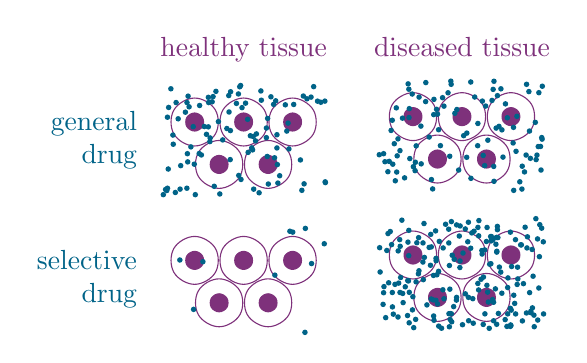
\begin{tikzpicture}[%
            hexagon/.style={regular polygon,regular polygon sides=6},
            cell/.pic={%
              \coordinate (-O) at (0,0);
              \node [%
                anchor=center,
                draw,
                hexagon,
                rounded corners=2em/4,
                minimum size=2em,
                inner sep=0pt,
                outer sep=2em/3,
                pic actions,
              ] (-wall) at (-O) {};
              \node [%
                anchor=center,
                fill,
                hexagon,
                rounded corners=0.8em/4,
                minimum size=0.8em,
                inner sep=0pt,
                outer sep=0pt,
                pic actions,
              ] (-nucleus) at (-O) {};
            },
            tissue/.pic={%
              \coordinate (-O) at (0,0);
              \pic (-cell 0) at (0,2em/3) {cell};
              \foreach \i in {3,...,6}
                \pic (-cell \i) at (-cell 0-wall.corner \i) {cell};
            }
          ]
            \node [palatinate] (healthy) {healthy tissue};
            \coordinate [below=2.5em of healthy] (healthy general);
            \coordinate [below=5em of healthy general] (healthy selective);
            \pic [palatinate] at (healthy selective) {tissue};
            \pic [palatinate] at (healthy general) {tissue};
            \foreach \x in {1,...,100}
              \fill [blue-palatinate] ($(1.5*2em*rand,2em*rand)+(healthy general)$) circle (0.1em);
            \foreach \x in {1,...,10}
              \fill [blue-palatinate] ($(1.5*2em*rand,2em*rand)+(healthy selective)$) circle (0.1em);

            \node [%
              palatinate,
              align=center,
              base right=1em of healthy,
            ] (diseased) {diseased tissue};
            \coordinate [below=2.5em of diseased] (diseased general);
            \coordinate [below=5em of diseased general] (diseased selective);
            \pic [palatinate] at (diseased selective) {tissue};
            \pic [palatinate] at (diseased general) {tissue};
            \foreach \x in {101,...,200}
              \fill [blue-palatinate] ($(1.5*2em*rand,2em*rand)+(diseased general)$) circle (0.1em);
            \foreach \x in {11,...,200}
              \fill [blue-palatinate] ($(1.5*2em*rand,2em*rand)+(diseased selective)$) circle (0.1em);

            \node [blue-palatinate,align=right,left=3.5em of healthy general] {general\\drug};
            \node [blue-palatinate,align=right,left=3.5em of healthy selective] {selective\\drug};
          \end{tikzpicture}
          \caption{Illustration of selective drug delivery.}
        \end{figure}
      \end{block}

    \column{0.5\textwidth}
      \begin{block}{Targets diseased tissue}
        \begin{itemize}
          \item<1-> Maximise therapeutic effects
          \item<1-> Minimise effective drug dose
        \end{itemize}
      \end{block}

      \begin{block}{Avoids healthy tissue}
        \begin{itemize}
          \item<1-> Minimise side-effects
        \end{itemize}
      \end{block}

  \end{columns}
\end{frame}

\subsection{Nanocarrier delivery systems}
\begin{frame}{\subsecname}
  \begin{itemize}
    \item<1-> pH
    \item<1->
  \end{itemize}
\end{frame}

\end{document}